\documentclass[10pt,a4paper]{article}
\usepackage[paper=a4paper, hmargin=3cm, bottom=3cm, top=3cm]{geometry}

\usepackage[utf8x]{inputenc}
\usepackage[spanish]{babel}

\usepackage{mathtools}
\usepackage{amsmath}
\usepackage{amsfonts}
\usepackage{amssymb}

\usepackage{xcolor}
\usepackage{listingsutf8}
\usepackage{booktabs}
\usepackage{hyperref}
\usepackage{multirow}

\usepackage{caption}
\usepackage{subcaption}

\usepackage{algorithm}
\usepackage[noend]{algpseudocode}

\usepackage{graphicx}
\usepackage{tikz}
\usepackage{relsize}
\usepackage{epstopdf}

\usepackage{bytefield}

\DeclarePairedDelimiter{\ceil}{\lceil}{\rceil}

% set the default code style
\lstset{
    frame=tb, % draw a frame at the top and bottom of the code block
    tabsize=4, % tab space width
    showstringspaces=false, % don't mark spaces in strings
    numbers=left, % display line numbers on the left
    commentstyle=\color{green}, % comment color
    keywordstyle=\color{blue}, % keyword color
    stringstyle=\color{red} % string color
}

% mathy stuff
\newtheorem{theorem}{Theorem}[section]
\newtheorem{lemma}[theorem]{Lemma}
\newtheorem{proposition}[theorem]{Proposición}
\newtheorem{corollary}[theorem]{Corollary}

\newenvironment{proof}[1][Demostración]{\begin{trivlist}
\item[\hskip \labelsep {\bfseries #1}]}{\end{trivlist}}
\newenvironment{definition}[1][Definición]{\begin{trivlist}
\item[\hskip \labelsep {\bfseries #1}]}{\end{trivlist}}
\newenvironment{example}[1][Example]{\begin{trivlist}
\item[\hskip \labelsep {\bfseries #1}]}{\end{trivlist}}
\newenvironment{remark}[1][Remark]{\begin{trivlist}
\item[\hskip \labelsep {\bfseries #1}]}{\end{trivlist}}

\newcommand{\qed}{\nobreak \ifvmode \relax \else
      \ifdim\lastskip<1.5em \hskip-\lastskip
      \hskip1.5em plus0em minus0.5em \fi \nobreak
      \vrule height0.75em width0.5em depth0.25em\fi}

\title{Teoría de las Comunicaciones \\ TP2}

\newcommand{\order}[1]{$\mathcal{O}(#1)$}

\begin{document}

%% cover page

\maketitle

\bigskip

\begin{table}[h]
\centering
\begin{tabular}{|l l l|}
\hline
Integrante       & \multicolumn{1}{c}{LU}     & Correo electrónico        \\ \hline
Martín Baigorria & \multicolumn{1}{c}{575/14} & martinbaigorria@gmail.com \\ 
Federico Beuter & 827/13                      & federicobeuter@gmail.com \\
Mauro Cherubini & 835/13                      & cheru.mf@gmail.com \\ \hline
\end{tabular}
\end{table}

\vfill

\begin{center}
\textbf{Reservado para la cátedra}
\end{center}
\begin{table}[h]
\centering
\begin{tabular}{|l|l|l|}
\hline
Instancia       & Docente & Nota \\ \hline
Primera entrega &         &      \\ \hline
Segunda entrega &         &      \\ \hline
\end{tabular}
\end{table}

\newpage
\tableofcontents
\newpage

% end cover page

\section{Introducción}

La comunicación es uno de los ejes fundamentales de la humanidad, a lo largo de la historia han aparecido diferentes medios para poder satisfacer esta necesidad, sin embargo el concepto nunca se habia formalizado. En 1948, el matemático e ingeniero Claude E. Shannon propone una definición formal de que es la comunicación desde una punto de vista matemático, donde origen a la \textit{Teoría de la Información}. En este trabajo analizaremos como aplica dicha teoria a un medio de comunicacion real, particularmente uno que sea altamente utilizado y tenga una alta densidad de usuarios.

\section{Desarrollo}

\subsection{Informacion y Entropia}

Como vimos en la introduccion, en 1948 el matematico Claude E. Shannon define formalmente que es la \textit{Informacion} en su publicacion \textit{A Mathematical Theory of Communication}, junto con esta defincion tambien introduce el concepto de \textit{Entropia} en la comunicacion. Primero definimos quienes son los participes en la comunicacion:

\begin{itemize}
	\item Fuente de Informacion
	\item Emisor
	\item Receptor
	\item Destino de Informacion
	\item Ruido
	\item Canal
\end{itemize}

Los mismos se encuentran conectados de la siguiente forma:

\begin{figure}[ht]
\begin{center}
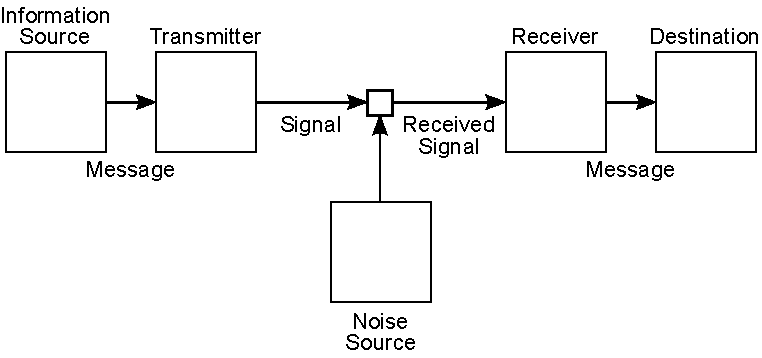
\includegraphics[width=0.6\columnwidth]{graficos/Shannon.pdf}
\caption{Diagrama de comunicacion}
\end{center}
\end{figure}

Para poder establecer una comunicacion punto a punto, es necesario que el emisor y el receptor "`hablen"' un lenguaje en comun. Para poder satisfacer esto, se define un conjunto de simbolos $S = \{ s_1, ..., s_n \}$, con una probabilidad $p(s_i)$ con $1 \leq i \leq n$ asociada a cada uno de ellos, este conjunto representa la totalidad de simbolos que pueden ser transmitidos por el canal. Una vez definido el conjunto, la informacion que se obtiene por simbolo es simplemente $I(s_i) = log(\frac{1}{p(s_i)})$. Se elige el logaritmo como funcion por cumplir con varias condiciones idóneas para calcular la informacion, de las mas interesantes tenemos que:

\begin{itemize}
	\item Si $s \in S$, entonces $I(s) \geq 0$
	\item Si $p(s_i) = 1$ para algun $i$, entonces $I(s_i) = 0$, ya que un evento que ocurre siempre no aporta información significativa
	\item $I(s_i, s_j) \leq I(s_i) + I(s_j)$, la igualdad vale unicamente si los simbolos son independientes
\end{itemize}

Como podemos apreciar, la funcion logaritmo cumple con todos estos puntos.

En nuestro trabajo analizaremos principalmente la entropia, esta se define como $H(S) = \sum\limits_{i=1}^n p(s_i)I(s_i)$. Esta medida representa la media de informacion obtenida por simbolo en la comunicacion, y se encuentra íntimamente relacionada con las probablidades de cada simbolo, particularmente mientras menos aleatoria sea una red, menor es la entropia. Tambien aplica el mismo razonamiento a la inversa, es decir, mientras mas cerca de la equiprobabilidad esten los simbolos, la entropia aumentara, maximizándose cuando los simbolos sean equiprobables.

%Antes de proceder a describir la metodologia para los experimentos, consideramos pertinente dar una interpretacion de la entropia. Podemos ver que esta medida esta relacionada con la probabilidad de cada simbolo, mientras menos informacion tengamos acerca de los símbolos, es natural asumir que estos se encuentran cerca de la equiprobabilidad. Sin embargo, a medida que tengamos mas conocimiento acerca de las posibilidades de aparición de cada símbolo, la entropia del canal va a bajar, ya que en los simbolos mas comunes no nos van aportar de informacion significativa. Esto lo podemos apreciar comparando los lenguajes basados en alfabeto reducido y los basados en pictogramas, si tomamos el caso del español que esta basado en el alfabeto latino, podemos ver que ciertas letras aparecen con mucho mas frecuencia que otras con lo cual la entropia tiende a ser menor, mientras que en el caso de lenguajes como el chino, al ser tan densos (el chino básico tiene hasta 50000 pictogramas) estimar las probabilidades se vuelve una tarea complicada, llevando a que la entropia sea mayor.

\subsection{Canal elegido}

Para poder tener suficientes datos para hacer un analisis interesante, seria prudente tomar un medio que sea ampliamente usado. Por ello, elegimos utilizar una red del tipo Wi-Fi, los puntos a destacar de la red son:

\begin{itemize}
	\item En la aplicaciones habituales, estas redes se caracterizan por tener un \textit{nodo} central, el cual se encarga de regular el trafico en la red
	\item En las redes publicas, los nodos que no son el central no se suelen comunicar entre ellos, estos principalmente se conectan con servidores en internet
\end{itemize}

\subsection{Paquetes de red}

En la redes la informacion en el canal se transmite en paquetes, estos paquetes tienen varios campos, particularmente nos interesan analizar los paquetes de capa 2 y capa 3. De los paquetes \textit{Ethernet} de capa 2, nos interesa:

\begin{itemize}
	\item Direccion MAC de origen
	\item Direccion MAC de destino
	\item Protocolo del payload, este depende del paquete de capa 3 que se esta transportando, puede ser IPv4, IPv6, ARP, etc.
\end{itemize}

Por otro lado, de los paquetes de capa 3 nos interesan solamente los ARP. De este tipo de paquetes nos interesan los campos:

\begin{itemize}
	\item Tipo de operacion
	\item Direccion MAC del emisor
	\item Direccion IP del emisor
	\item Direccion MAC del destinatario
	\item Direccion IP del destinatario
\end{itemize}

El fin de los paquetes ARP, es vincular la capa 2 con la capa 3, relacionando las direcciones IP con direcciones MAC fisicas. Para hacer esto el protocolo ARP cuenta con dos operaciones, estas pueden ser \textit{who-has} o \textit{is-at}.

Las operaciones \textit{who-has} sirven para identificar a que direccion MAC fisica corresponda una direccion IP de la red, estos paquetes suelen ser de tipo \textit{broadcast}.

En respuesta a los \textit{who-has}, tenemos las operaciones \textit{is-at}. Una vez que un nodo recibe un paquete de tipo \textit{who-has}, este revisa si la direccion IP del mismo coincide con la suya, en el caso de que lo sea este envia un paquete al nodo que genero el \textit{who-has} para notificarle su direccion MAC fisica.

Para no tener que enviar paquetes ARP por cada paquete IP que se desea enviar, el emisor del \textit{who-has} al recibir el \textit{is-at}, guarda el resultado en una tabla para poder enviar futuros paquetes al mismo destino inmediatamente.

\section{Metodologia}

En el trabajo se pide que analicemos dos fuentes de informacion, estas son $S$ y $S_1$, y tienen la siguiente forma:

\begin{itemize}
	\item $S$: Comprende a todos los paquetes \textit{Ethernet} que circulan por el canal, se los diferencia por el \textit{protocolo} del payload.
	\item $S_1$: Se limita a los paquetes \textit{Ethernet} de tipo ARP.
\end{itemize}

\pagebreak

Para $S_1$ ademas se pide establecer un criterio de diferenciacion, para esto tomamos la conjuncion de las direcciones IP fuente y destino de los paquetes ARP de tipo \textit{who-has}. Elegimos estos paquetes ya que los \textit{is-at} se dan unicamente en respuesta a algun \textit{who-has} anterior, con lo cual estariamos duplicando ciertos paquetes.

Las redes elegidas para \textit{sniffear} fueron las siguientes:

\begin{itemize}
	\item FibertelZone, en shopping Plaza Oeste Moron (60 min. de captura)
	\item Laboratorios-DC (30 min. de captura)
\end{itemize}

Inicialmente la idea era capturar paquetes en una mayor cantidad de redes, sin embargo, nos topamos con que en diferentes redes publicas el trafico no era suficientemente alto, con lo cual la captura de paquetes no era significativa ni suficiente como para hacer un analisis mas exhaustivo. Consideramos que esto se debe en parte al aumento en el uso de Smartphones con redes moviles, junto con la mala fama que tienen las redes Wi-Fi publicas.

\section{Resultados}

\subsection{Protocolos}

Vamos a ver primero la cantidad de paquetes en las redes:

\begin{figure}[ht]
\begin{center}
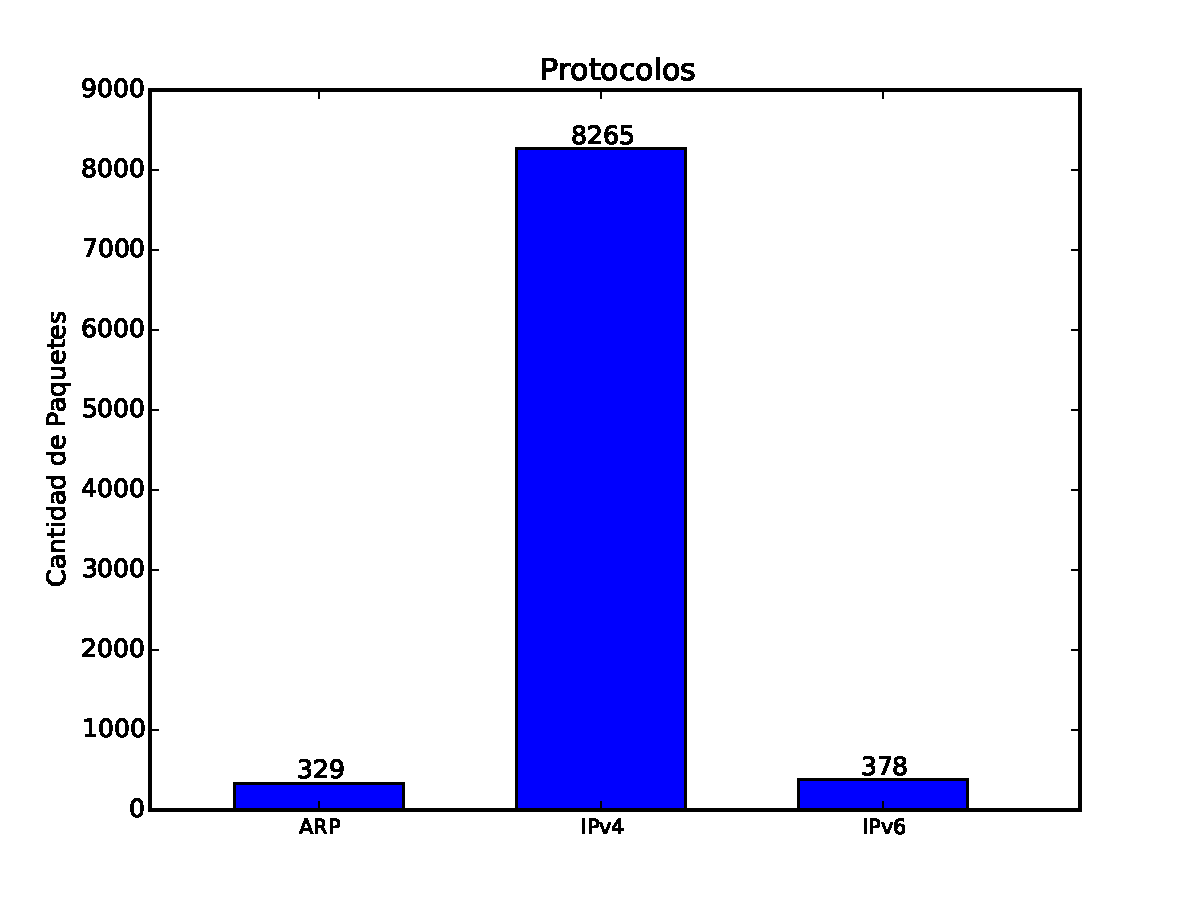
\includegraphics[width=0.8\columnwidth]{graficos/plaza_s1.pdf}
\caption{Red Plaza Oeste}
\end{center}
\end{figure}

\begin{figure}[ht]
\begin{center}
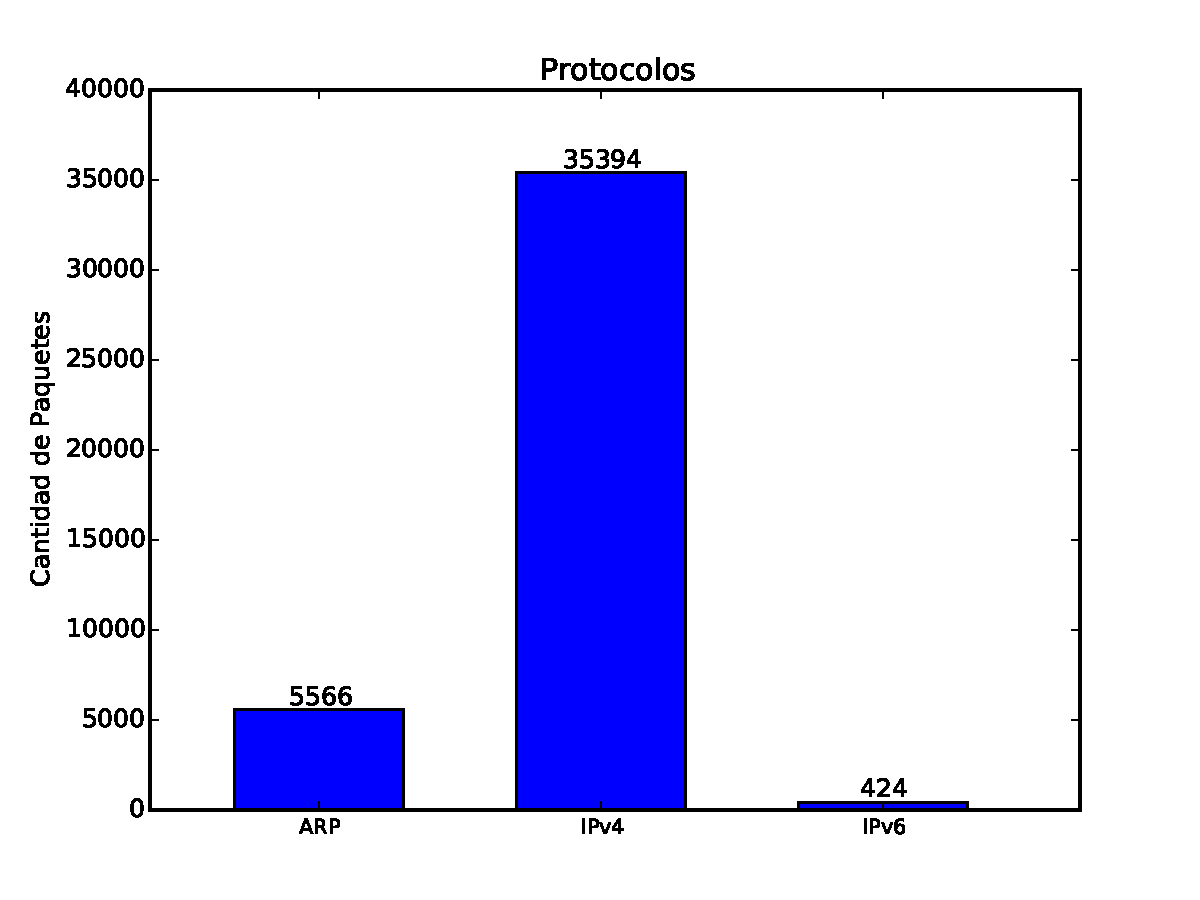
\includegraphics[width=0.6\columnwidth]{graficos/dc_s1.pdf}
\caption{Red Laboratorios DC}
\end{center}
\end{figure}

\pagebreak

Como podemos apreciar, los paquetes IPv4 dominan el trafico de la red. A continuacion vamos a ver la informacion por simbolo junto con la entropia:

\begin{figure}[ht]
\begin{center}
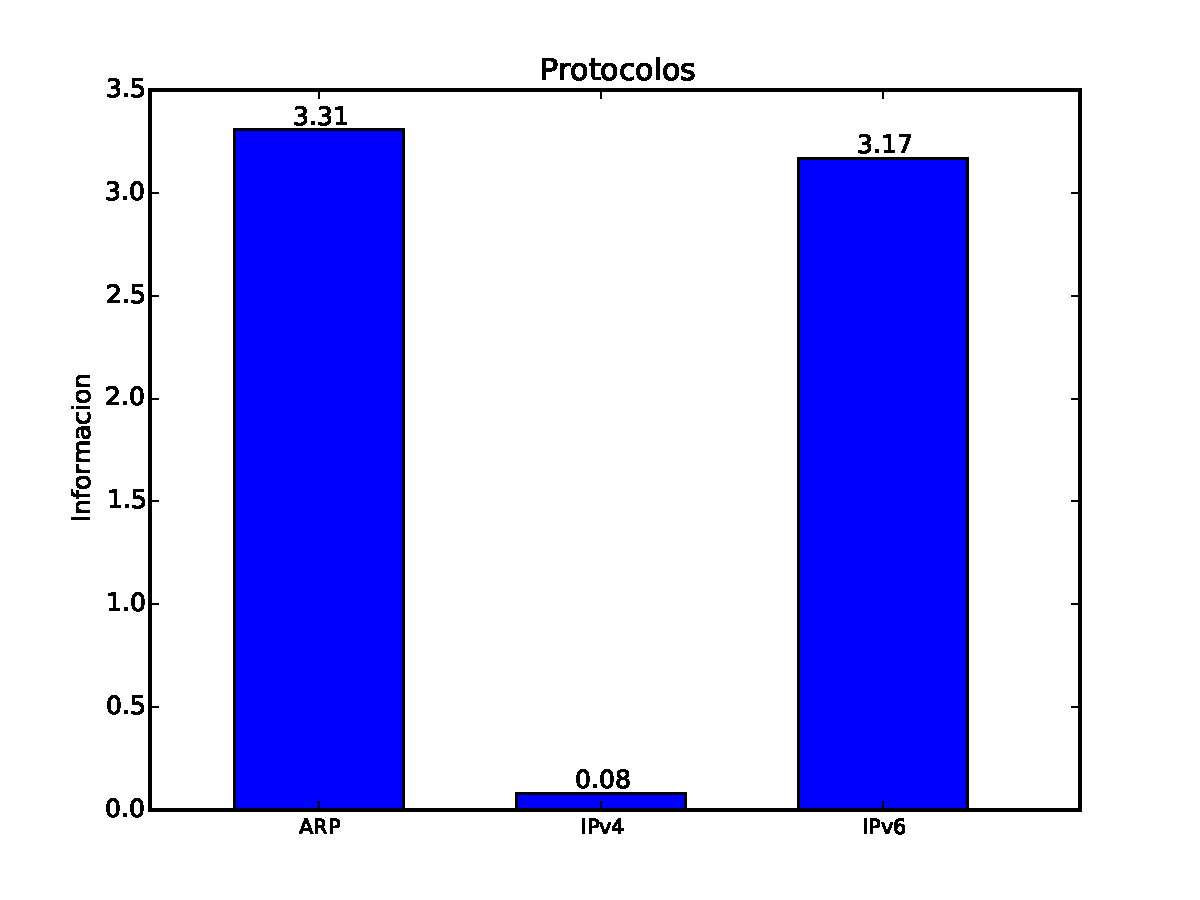
\includegraphics[width=0.6\columnwidth]{graficos/plaza_inf_s1.pdf}
\caption{Red Plaza Oeste}
\end{center}
\end{figure}

\begin{figure}[ht]
\begin{center}
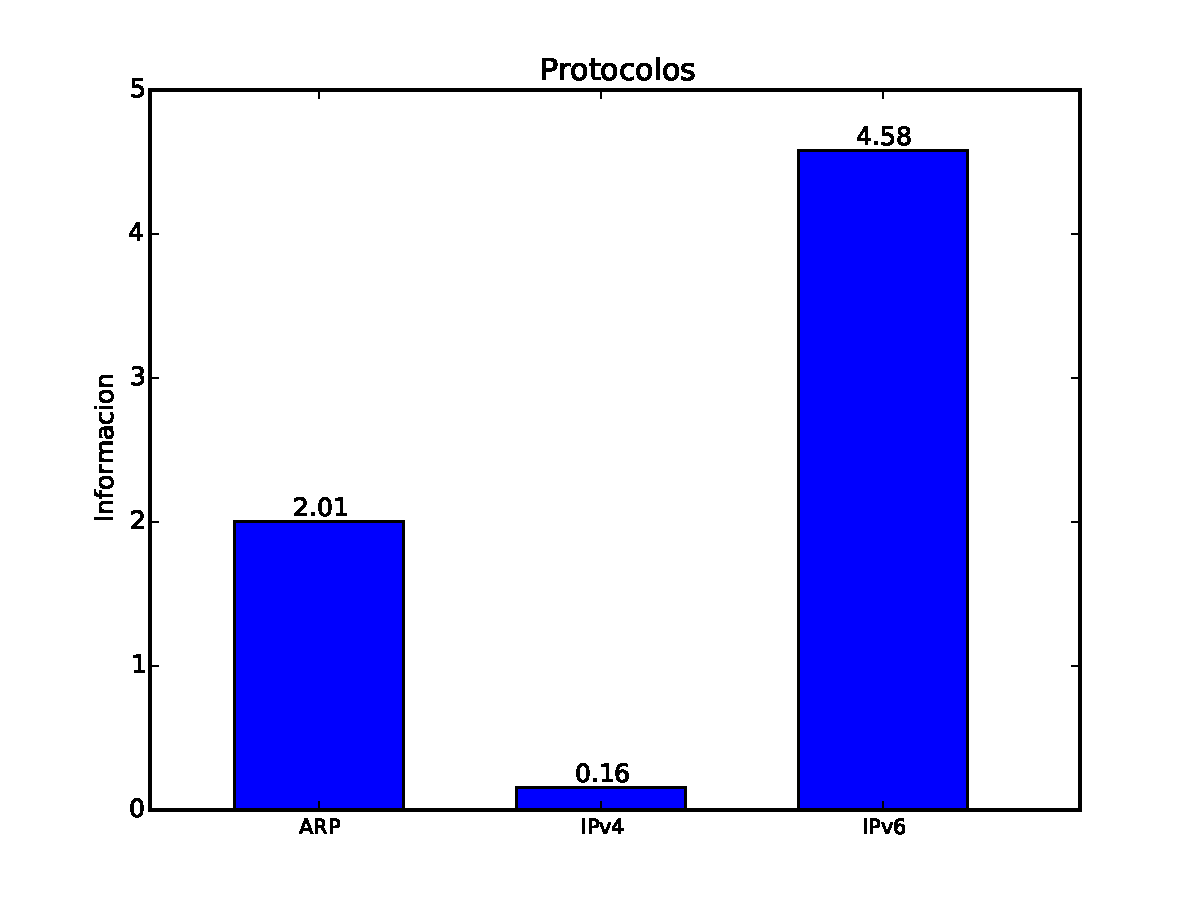
\includegraphics[width=0.8\columnwidth]{graficos/dc_inf_s1.pdf}
\caption{Red Laboratorios DC}
\end{center}
\end{figure}

\pagebreak

La entropia en las redes fue:

\begin{table}[ht]
\centering
\caption{Entropia}
\label{my-label}
\begin{tabular}{ll}
\hline
Red         & Entropia \\ \hline
Plaza Oeste & 0.3303   \\
Laboratorios DC    & 0.4505   \\ \hline
\end{tabular}
\end{table}

Como podemos ver, la entropia de la red es bastante baja en ambos, esto se debe a la gran cantidad de paquetes IPv4 en ambos canales. Otro punto interesante es que en la red unicamente circulan paquetes de tipo ARP, IPv4 o IPv6, si bien esto es esperable en la red del Plaza Oeste nos sorprendió que ocurra también en la red Laboratorios DC, asumimos que allí podríamos encontrar en uso algún protocolo mas esotérico.

Nuestras predicciones indicaban que la mayoría de los paquetes iban a ser de tipo IPv4 por un margen bastante significativo, esto se corresponde con que la probabilidad de dicho paquete iba a ser mucho mas alta que el resto, con lo cual la información de dichos paquetes iba a ser considerablemente menor. Como la diferencia es tan amplia, por un margen muy significativo, consideramos al protocolo IPv4 como símbolo distinguido.

\pagebreak

\subsection{Paquetes ARP}

Como vimos en el desarrollo, definimos los símbolos de $S_1$ como las direcciones IP de origen y destino de los paquetes ARP. Por motivos de presentación, nos limitamos a graficar unicamente las diez direcciones que mas aparecieron durante el \textit{sniffeo}. Los resultados fueron:


\begin{figure}[ht]
\begin{center}
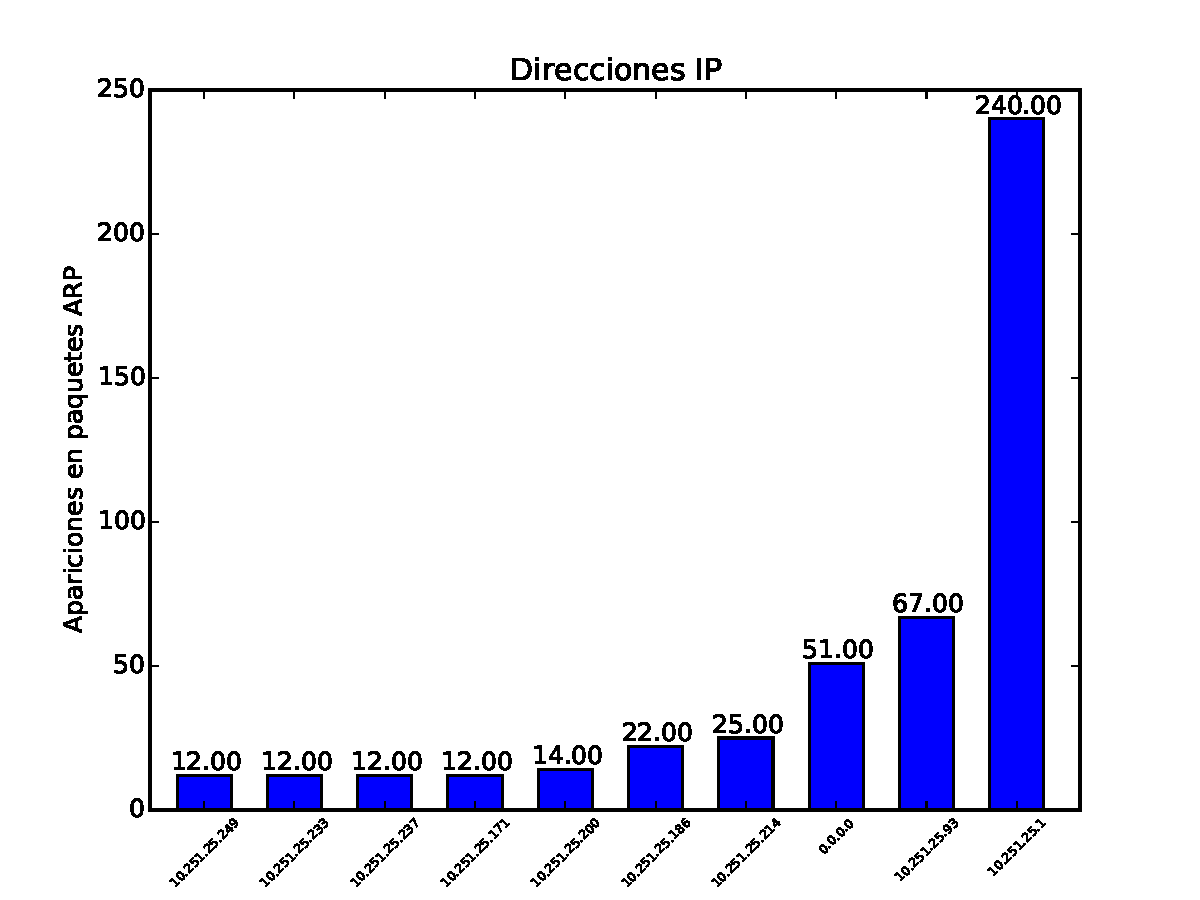
\includegraphics[width=0.6\columnwidth]{graficos/plaza_top_s2.pdf}
\caption{Red Plaza Oeste}
\end{center}
\end{figure}

\begin{figure}[ht]
\begin{center}
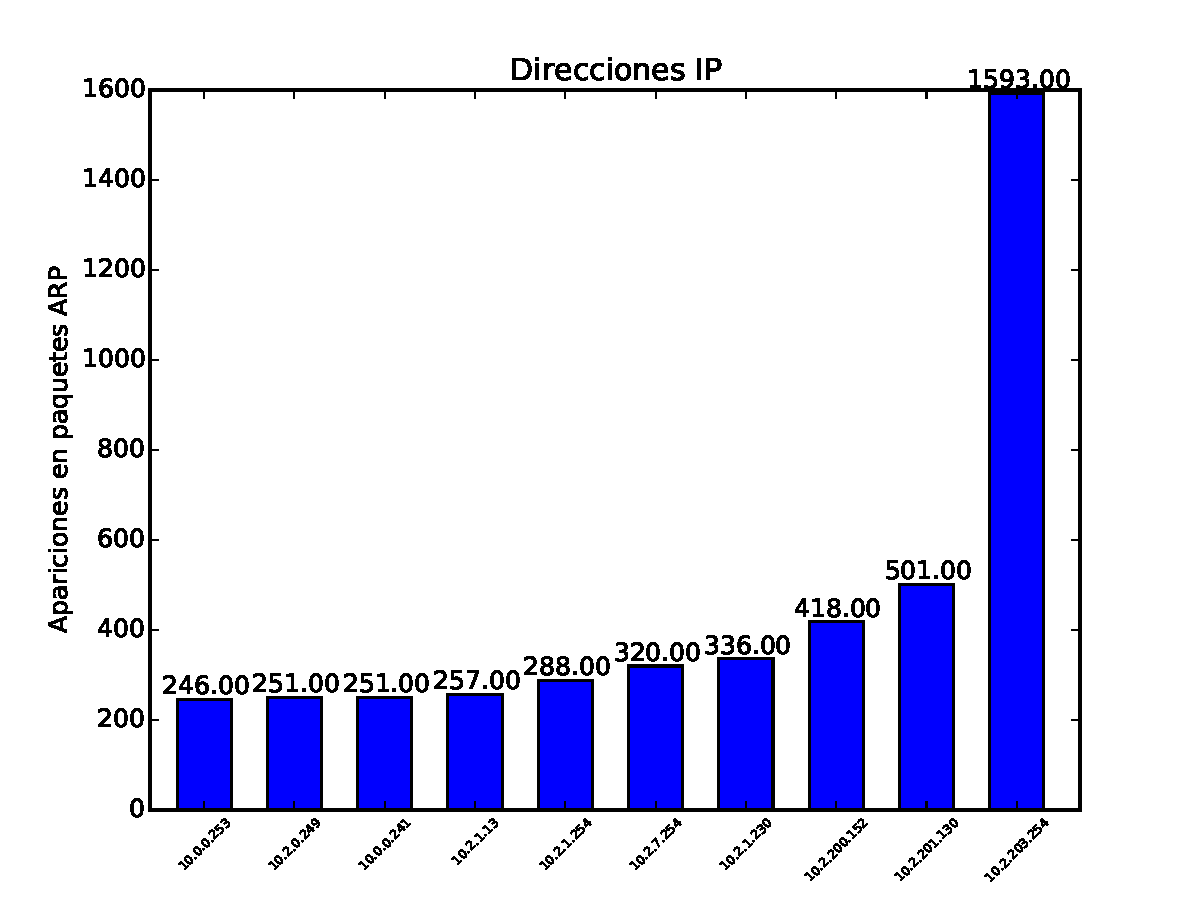
\includegraphics[width=0.6\columnwidth]{graficos/dc_top_s2.pdf}
\caption{Red Laboratorios DC}
\end{center}
\end{figure}

\pagebreak

Una de las suposiciones que teníamos, era que por el funcionamiento de la red Wi-Fi, la gran mayoría de los paquetes irían dirigidos hacia un nodo principal, el cual después se encargaría de redirigirlos al destino apropiado. Como podemos ver, esto ocurrió en ambos casos, hay un nodo el cual tiene muchas mas apariciones que el resto.

A pesar de que los resultados satisfacían nuestras teorías, nos sorprendió que el margen de diferencia entre el nodo principal y el resto no sea mayor, con lo cual los otros nodos también están enviando paquetes ARP a nodos que no son el principal. Esto sera estudiado mas adelante, primero vamos a ver la información en ambos canales, nuevamente limitándonos a las diez direcciones que mas aparecieron:

\begin{figure}[ht]
\begin{center}
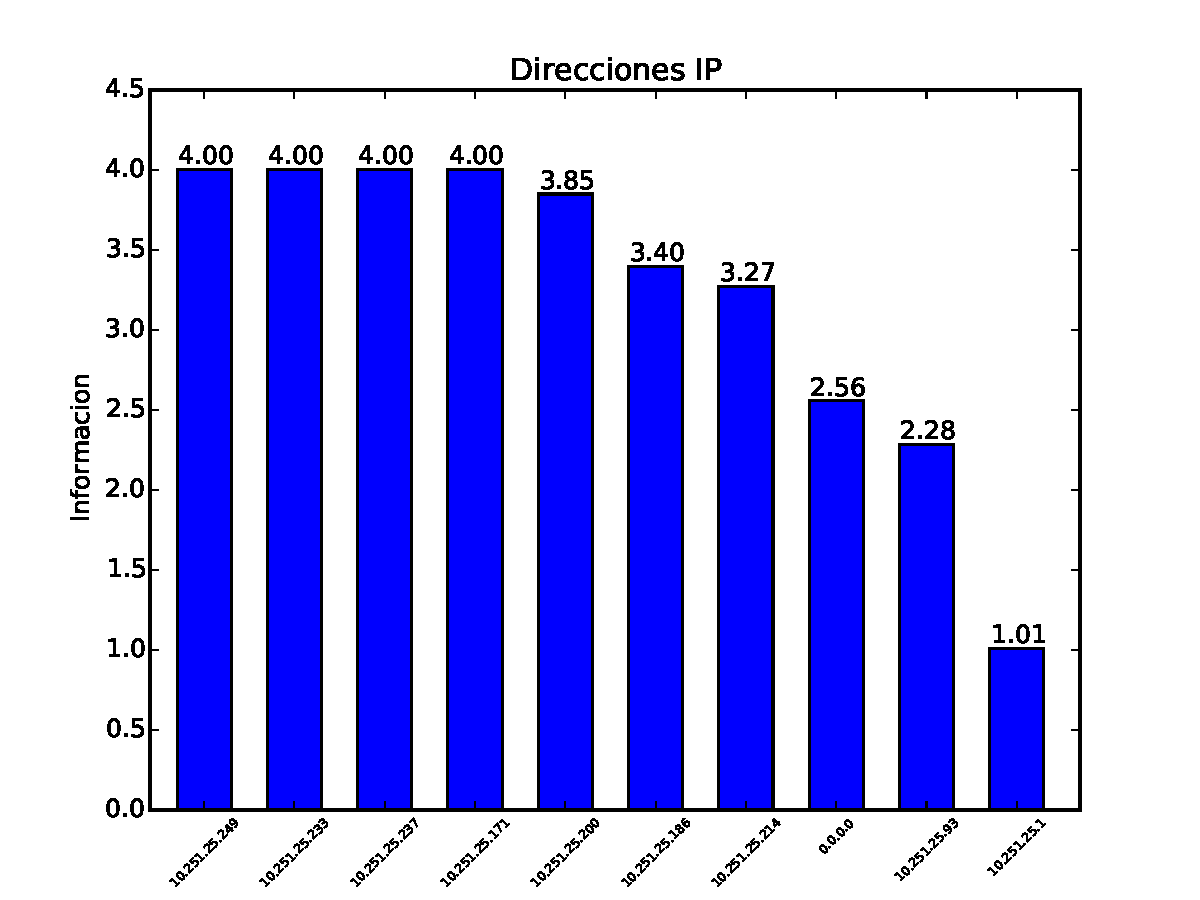
\includegraphics[width=0.6\columnwidth]{graficos/plaza_top_inf_s2.pdf}
\caption{Red Plaza Oeste}
\end{center}
\end{figure}

\begin{figure}[ht]
\begin{center}
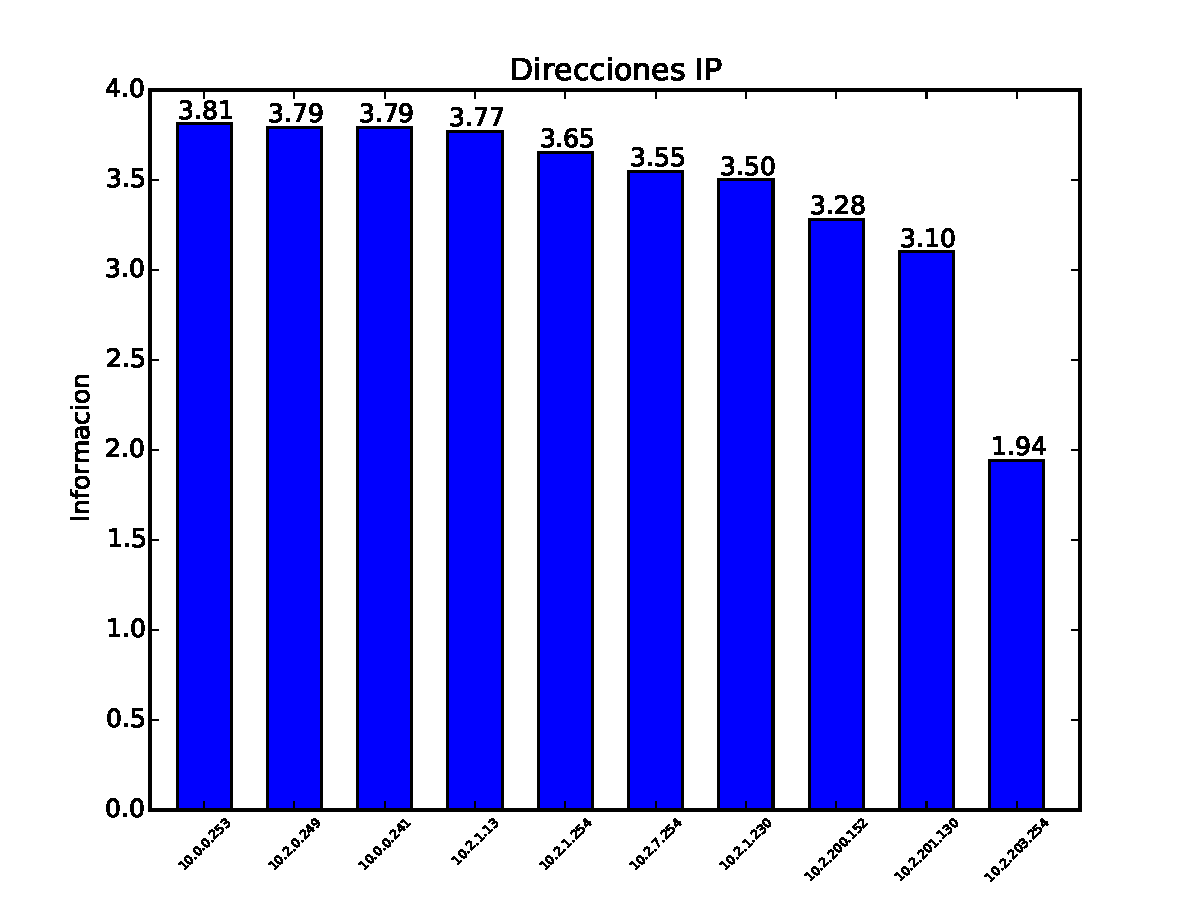
\includegraphics[width=0.6\columnwidth]{graficos/dc_top_inf_s2.pdf}
\caption{Red Laboratorios DC}
\end{center}
\end{figure}

\pagebreak

La entropia para estas dos redes fue:

\begin{table}[ht]
\centering
\caption{Entropia}
\label{my-label}
\begin{tabular}{ll}
\hline
Red         & Entropia \\ \hline
Plaza Oeste & 3.1724   \\
Laboratorios DC    & 4.6459   \\ \hline
\end{tabular}
\end{table}

Una cosa interesante a destacar, es que la entropia es mucho mayor tomando como símbolos las direcciones IP que los tipos de protocolos, esto ocurre en ambas redes. Esto creemos que se debe principalmente a las siguientes razones:

\begin{itemize}
	\item La cantidad de protocolos es considerablemente menor que la cantidad de direcciones IP posibles, en la practica unicamente vimos tres protocolos en uso
	\item En las redes Wi-Fi, vimos que los nodos que suelen enviar paquetes de tipo \textit{who-has} son aquellos que quieren conectarse a la red, estos suelen tener direcciones IP diferentes a las que ya se encuentran en el sistema, con lo que tenemos que agregar un nuevo símbolo
	\item Es posible que el tamaño de la muestra no haya sido suficiente, y que se necesiten mas tiempo de \textit{sniffeo} para poder calcular bien la entropia
\end{itemize}

Este ultimo punto es particularmente interesante para nosotros, ya que es posible que la muestra tomada no sea significativa del trafico de la red y no sea suficiente para estimar las probabilidades, efectivamente afectando la entropia de la red. También seria interesar estudiar si las políticas de asignación de IP de la red y el uso de la misma terminan amortizando el segundo punto, ya que si el sistema reasigna direcciones siempre que puede, mientras mas grande sea la muestra la diferencia entre el nodo principal y el resto potencialmente seria mayor.

En general, la red respondió de la manera que esperábamos, pudimos identificar un nodo principal el cual aparece en muchas mas ocasiones que el resto en ambas redes. Si bien la diferencia en cantidad de apariciones de dichos nodos respecto al resto no fue tan significativa, creemos que fue suficiente como para marcarlos como símbolos distinguidos en sus respectivos canales.

\subsection{Paquetes de control ARP}

En la sección anterior hablamos de paquetes que no eran enviados hacia el nodo principal, ademas de esto, nos dimos cuenta que varios de ellos tenian una forma bastante particular, tras consultar diferentes recursos nos dimos cuenta que varios de ellos eran paquetes de control. Nos topamos con los siguientes:

\begin{itemize}
	\item Dirección IP \texttt{0.0.0.0}: Estos paquetes se utilizan para revisar si una dirección IP se encuentra en uso por algún host, la idea es que un nodo al recibir una dirección IP para usar, envia este paquete, y si recibe un \textit{is-at} de otro nodo quiere decir que la dirección que pretendía utilizar esta en uso
	\item Misma dirección IP de fuente y destino: Este es un paquete bastante particular, sirve para que los diferentes hosts en la red tengan sus tablas de dirección IP y MAC actualizadas. La idea es que al recibir el paquete y verificar que las direcciones origen y destino son iguales, el host revisa si tiene la dirección MAC en su tabla, en caso de tenerla actualiza la dirección IP almacenada si es que esta cambio por la dirección que figura en el paquete. Mantener las relaciones IP y MAC actualizadas es sumemente importante en la red, ya que eso puede ahorrarnos una cantidad significativa de tiempo a la hora de manejar el trafico.
\end{itemize}

Las apariciones de estos paquetes consideramos que terminaron quitandole bastante peso al nodo central respecto a los demás, haciendo que la entropia sea mayor.

\section{Conclusiones}

Es bastante interesante ver como los diferentes conceptos de teoria de la informacion aplican en canales reales, particularmente considerando que fueron planteados en 1948 cuando las redes modernas no existian. Desde el punto de vista de las redes Wi-Fi puntualmente, vimos como la comunicacion es sumamente centralizada y dominada por IPv4, lo primero se puede ver claramente en los paquetes ARP los cuales en nuestras muestras estan en gran parte dirigidos a un unico nodo, mientras que lo segundo no solamente se ve a simple vista, sino que ademas es esperable considerando que la Internet funciona sobre IPv4.

Como estudio a futuro, seria interesante hacer un \textit{sniffeo} durante el lapso de uno o mas dias, para poder ver si las proporciones obtenidas con la fuente $S_1$ se mantienen, o si eventualmente el nodo principal se impone respecto al resto aumentando aun mas la diferencia entre estos.

%\subsection{Proporcion de trafico local e Internet}
%
%METER ESTO EN DISTINCION DE NODOS
%
%Nos parecio tambien interesante analizar la proporcion de trafico local respecto al trafico que va hacia Internet, nuestra teoria es que en la red publica del Plaza Oeste todo el trafico se destina a Internet a traves del enrutador. Por otro lado, la red Laboratorios-DC, al ser de la facultad, seguramente tengo mas trafico interno.
\newpage
\input{desarrollo}
\newpage
\section{Traceroute a Universidades}

A continuacion mostramos diferentes traceroutes a universidades. El RTT promedio se calculo a partir de 5 requests. El host name lo conseguimos a partir de la funcion socket.gethostbyaddr de Python, que lo que hace es simplemente un DNS lookup. La ubicación la conseguimos a partir de una base de datos publica de GeoIP.

\subsection{dc.ubar.ar}

\begin{table}[H]
\centering
\caption{traceroute: dc.uba.ar}
\begin{tabular}{@{}lllll@{}}
\toprule
Hop & Avg. RTT & IP Address & Host name & Location\\ \midrule
1 & 9.3842 ms & 181.169.12.1 & 1-12-169-181.fibertel.com.ar & AR, SA\\
2 &  * * * * * &  &  &  \\
3 &  * * * * * &  &  &  \\
4 &  * * * * * &  &  &  \\
5 & 14.025 ms & 200.89.164.53 & 53-164-89-200.fibertel.com.ar & AR, SA\\
6 & 14.7514 ms & 200.89.165.2  & 2-165-89-200.fibertel.com.ar & AR, SA\\
7 & 22.5916 ms & 200.89.165.86 & 86-165-89-200.fibertel.com.ar & AR, SA\\
8 & 16.5408 ms & 200.49.69.161 & VPN-corp.metrored.net.ar & AR, SA\\
9 &  * * * * * &  &  &  \\
10 &  * * * * * &  &  &  \\
11 &  * * * * * &  &  &  \\
12 & 12.7052 ms & 157.92.47.53 & 157.92.47.53 & AR, SA\\
13 & 13.067 ms & 192.168.121.2 & 192.168.121.2 &  \\
14 &  * * * * * &  &  &  \\
... &  * * * * * &  &  &  \\

 \bottomrule
\end{tabular}
\label{dc}
\end{table}

Como es de esperar, al hacer un request a dc.uba.ar desde Argentina no hay saltos intercontinentales. Sin embargo, notemos que este traceroute cae en el problema de missing destination. Esto no es porque el servidor no exista, si no porque probablemente esta configurado para no devolver ICMP requests.

Intentamos acceder a metrored.net.ar, ya sea por URL o por IP y no lo logramos. Sin embargo, al hacer un IP Whois encontramos:

\begin{table}[H]
\centering
\caption{Whois lookup: metrored.net.ar}
\begin{tabular}{@{}ll@{}}
\toprule
owner:       &   Techtel LMDS Comunicaciones Interactivas S.A. \\
ownerid:     &   AR-TLCI-LACNIC \\
responsible: & Administrador de Direcciones IP - CLARO \\
address:     &   Garay, 34 \\
address:     &   C1063AB - Buenos Aires \\
country:     &   AR \\
phone:       &   +54 11 4000-3000 [3270] \\
nserver:     &   DNSMR1.METRORED.NET.AR   \\ \bottomrule
\end{tabular}
\end{table}

Por lo que podemos ver, el hop pertenece a Claro.

\subsection{mit.edu}

\begin{table}[H]
\caption{traceroute: mit.edu}
\centering
\begin{tabular}{@{}lllll@{}}
\toprule
Hop & Avg. RTT & IP Address & Host name & Location\\ \midrule
1 & 12.6968 ms & 181.169.12.1 & 1-12-169-181.fibertel.com.ar & AR, SA\\
2 &  * * * * * &  &  &  \\
3 &  * * * * * &  &  &  \\
4 &  * * * * * &  &  &  \\
5 & 20.0602 ms & 200.89.160.9 & 9-160-89-200.fibertel.com.ar & AR, SA\\
6 & 18.026 ms & 200.89.165.198 & 198-165-89-200.fibertel.com.ar & AR, SA\\
7 & 13.8548 ms & 200.89.165.86 & 86-165-89-200.fibertel.com.ar & AR, SA\\
8 & 13.0754 ms & 195.22.220.154 & xe-1-2-0.baires3.bai.seabone.net & IT, EU\\
9 & 251.8128 ms & 149.3.183.73 & 149.3.183.73 & IT, EU\\
10 & 254.8316 ms & 89.221.43.107 & akamai-row.londra32.lon.seabone.net & IT, EU\\
11 & 253.6456 ms & 104.65.21.108 & a104-65-21-108.deploy.static.akamaitechnologies.com & NL, EU\\\bottomrule
\end{tabular}
\label{mit}
\end{table}

En este gráfico hay un enlace transatlántico claramente identificable entre el hop 7 y el hop 8. Notar que el host name ya indica que es transatlántico. Buscando a quien pertenece seabone.net, averiguamos que pertenece a la empresa Sparkle que provee servicios de enlaces transatlánticos.

\begin{tcolorbox}
Sparkle is a leading global telecommunication service provider, offering a complete range of IP, Data, Cloud, Data Center, Mobile and Voice solutions designed to meet the ever changing needs of Fixed and Mobile Operators, ISPs, OTTs, Media \& Content Players, Application Service Providers and Multinational Corporations (MNCs)
\end{tcolorbox}

Curiosamente, al final el request termino en Holanda en nodo de Akamai y no en Estados Unidos. Haciendo un Whois al URL confirmamos que esto es correcto.

\subsection{ox.ac.uk}

\begin{table}[H]
\caption{traceroute: ox.ac.uk (oxford)}
\centering
\begin{tabular}{@{}lllll@{}}
\toprule
Hop & Avg. RTT & IP Address & Host name & Location\\ \midrule
1 & 10.9412 & 181.169.12.1 ms & 1-12-169-181.fibertel.com.ar & AR, SA\\
2 &  * * * * * &  &  &  \\
3 &  * * * * * &  &  &  \\
4 &  * * * * * &  &  &  \\
5 & 16.9558 & 200.89.160.13 ms & 13-160-89-200.fibertel.com.ar & AR, SA\\
6 & 15.4314 & 200.89.165.250 ms & 250-165-89-200.fibertel.com.ar & AR, SA\\
7 & 9.7228 & 190.216.88.33 ms & 190.216.88.33 & AR, SA\\
8 & 138.7252 & 67.17.99.233 ms & ae0-300G.ar5.MIA1.gblx.net & US, NA\\
9 &  * * * * * &  &  &  \\
10 &  * * * &  &  &  \\
10 & 224.1195 & 4.69.143.190 ms & ae-1-3104.ear2.London2.Level3.net & US, NA\\
11 & 224.8286 & 212.187.139.166 ms & unknown.Level3.net & GB, EU\\
12 & 236.9458 & 146.97.33.2 ms & ae29.londpg-sbr2.ja.net & GB, EU\\
13 & 240.9694 & 146.97.37.194 ms & ae19.readdy-rbr1.ja.net & GB, EU\\
14 & 227.1278 & 193.63.108.94 ms & ae2.oxfoii-rbr1.ja.net & GB, EU\\
15 & 227.3266 & 193.63.108.98 ms & ae3.oxforq-rbr1.ja.net & GB, EU\\
16 & 228.0936 & 193.63.109.90 ms & 193.63.109.90 & GB, EU\\
17 &  * * * * * &  &  &  \\
18 &  * * * * * &  &  &  \\
19 & 239.6874 & 192.76.32.62 ms & boucs-lompi1.sdc.ox.ac.uk & GB, EU\\
20 & 225.6974 & 129.67.242.154 ms & aurochs-web-154.nsms.ox.ac.uk & GB, EU\\ \bottomrule
\end{tabular}
\label{oxford}
\end{table}

Aquí podemos identificar claramente enlaces transatlánticos a partir del host name y la ubicación. Level3 es una empresa conocida proveedora de enlaces. Un dato de color, sus acciones cotizan en Nasdaq.

\begin{tcolorbox}
Level 3 Communications, Inc. is a premier provider of global communication services, creating solutions that strengthen the growth, efficiency and security of businesses around the world. Our business started as part of a subsidiary of a construction company that created one of the first competitive local exchange carriers, MFS Communications.
\end{tcolorbox}

\subsection{u-tokyo.ac.jp}

\begin{table}[H]
\caption{traceroute: u-tokyo.ac.jp}
\centering
\begin{tabular}{@{}lllll@{}}
\toprule
Hop & Avg. RTT & IP Address & Host name & Location\\ \midrule
1 & 9.9508 ms & 181.169.12.1 & 1-12-169-181.fibertel.com.ar & AR, SA\\
2 &  * * * * * &  &  &  \\
3 &  * * * * * &  &  &  \\
4 &  * * * * * &  &  &  \\
5 & 16.979 ms & 200.89.160.21 & 21-160-89-200.fibertel.com.ar & AR, SA\\
6 & 15.2796 ms & 200.89.165.222 & 222-165-89-200.fibertel.com.ar & AR, SA\\
7 & 10.541 ms & 195.22.220.102 & xe-1-0-3.baires5.bai.seabone.net & IT, EU\\
8 & 39.8348 ms & 195.22.219.17 & ae7.sanpaolo8.spa.seabone.net & IT, EU\\
9 & 36.1798 ms & 195.22.219.17 & ae7.sanpaolo8.spa.seabone.net & IT, EU\\
10 & 42.7854 ms & 149.3.181.65 & 149.3.181.65 & IT, EU\\
11 & 159.2136 ms & 129.250.2.227 & ae-4.r24.nycmny01.us.bb.gin.ntt.net & US, NA\\
12 & 237.3446 ms & 129.250.4.13 & ae-2.r20.sttlwa01.us.bb.gin.ntt.net & US, NA\\
13 & 225.4494 ms & 129.250.2.54 & ae-0.r21.sttlwa01.us.bb.gin.ntt.net & US, NA\\
14 & 426.808 ms & 129.250.3.86 & ae-2.r20.osakjp02.jp.bb.gin.ntt.net & US, NA\\
15 & 429.0596 ms & 129.250.6.188 & ae-4.r22.osakjp02.jp.bb.gin.ntt.net & US, NA\\
16 & 421.2708 ms & 129.250.2.255 & ae-1.r01.osakjp02.jp.bb.gin.ntt.net & US, NA\\
17 & 417.919 ms & 61.200.80.218 & xe-0-4-0-7.r01.osakjp02.jp.ce.gin.ntt.net & JP, AS\\
18 & 425.9262 ms & 158.205.192.173 & ae0.ostcr01.idc.jp & JP, AS\\
19 & 426.6464 ms & 158.205.192.86 & 158.205.192.86 & JP, AS\\
20 & 534.723 ms & 158.205.121.250 & po2.l321.fk1.eg.idc.jp & JP, AS\\
21 & 436.512 ms & 154.34.240.254 & 154.34.240.254 & JP, AS\\
22 & 424.7352 ms & 210.152.135.178 & 210.152.135.178 & JP, AS\\
 \bottomrule
\end{tabular}
\label{tokyo}
\end{table}

\vspace{1px}

Como era de esperar, este termino siendo el traceroute mas largo, pasando por un camino sumamente raro. De Argentina a Italia, luego a EE.UU. y finalmente a Japón. Sin embargo, si vemos esto desde un punto de vista económico tiene sentido. El trafico desde América Latina a Japon no debe ser muy alto, por lo que no se justifican los altos costos de hacer un enlace mas directo.

Encontramos nuevamente los enlaces transatlánticos de Sparkle. Entrando a ntt.net nos encontramos con:


\includegraphics[width=\textwidth,keepaspectratio]{images/ntt}

Esto nos hace inferir que es una empresa Japonesa de telecomunicaciones.
\newpage
\section{Experimentos}

Recordar decir como mido el RTT!

\subsection{Caching}

\begin{table}[H]
\caption{traceroute: google.com sin caching}
\centering
\begin{tabular}{@{}lllll@{}}
\toprule
Hop & Avg. RTT & IP Address & Host name & Location\\ \midrule
1 & 10.6688 ms & 181.169.12.1 & 1-12-169-181.fibertel.com.ar & AR, SA\\
2 &  * * * * * &  &  &  \\
3 &  * * * * * &  &  &  \\
4 &  * * * * * &  &  &  \\
5 & 20.2096 ms & 200.89.160.21 & 21-160-89-200.fibertel.com.ar & AR, SA\\
6 & 14.3278 ms & 200.89.165.129 & 129-165-89-200.fibertel.com.ar & AR, SA\\
7 & 12.5566 ms & 200.89.165.150 & 150-165-89-200.fibertel.com.ar & AR, SA\\
8 &  * * * * * &  &  &  \\
9 & 10.9052 ms & 209.85.251.86 & 209.85.251.86 & US, NA\\
10 & 40.759 ms & 209.85.252.42 & 209.85.252.42 & US, NA\\
11 & 38.5816 ms & 216.239.58.221 & 216.239.58.221 & US, NA\\
12 & 38.1802 ms & 216.58.202.4 & gru06s26-in-f4.1e100.net & US, NA\\ \bottomrule
\end{tabular}
\label{google}
\end{table}


\begin{table}[H]
\caption{traceroute: google.com con caching}
\centering
\begin{tabular}{@{}lllll@{}}
\toprule
Hop & Avg. RTT & IP Address & Host name & Location\\ \midrule
1 & 11.1854 ms & 181.169.12.1 & 1-12-169-181.fibertel.com.ar & AR, SA\\
2 &  * * * * * &  &  &  \\
3 &  * * * * * &  &  &  \\
4 &  * * * * * &  &  &  \\
5 & 21.9184 ms & 200.89.165.33 & 33-165-89-200.fibertel.com.ar & AR, SA\\
6 & 15.066 ms & 200.89.164.26 & 26-164-89-200.fibertel.com.ar & AR, SA\\
7 &  * * * * * &  &  &  \\
8 & 11.6574 ms & 181.30.241.187 & 187-241-30-181.fibertel.com.ar & AR, SA\\ \bottomrule
\end{tabular}
\label{googlecache}
\end{table}

\subsection{Detección de links intercontinentales}

1. Falsos Positivos / Falsos Negativos


            Intercontinental     Local
Test Intercontinental
Test Local

Muestra: 100 sitios de alexa?

Hacer funcion que detecte enlaces intercontinentales con libreria de Python.

\subsection{Traceroute anomalities}


\newpage
\section{Conclusión}

Poder trazar la ruta que un paquete potencialmente puede tomar es sumamente importante, particularmente para podes identificar saltos donde la red se puede congestionar o tener errores. Esta funcionalidad es ampliamente utilizada a día de hoy, si bien en este trabajo practico vimos un método para la implementación de esta herramienta, existen otras maneras de implementarla.

El método propuesto en el TP consiste en abusarse de los paquetes ICMP para poder obtener la ruta del origen al destino, el problema de esto es que es posible que la ruta cambie durante la ejecución obteniendo así una ruta invalida (es una posibilidad minima que puede ser mitigada fácilmente ejecutando varias veces el algoritmo), en varias ocasiones se contemplo incluir la traza de rutas en los protocolos y paquetes, un método fue propuesto en el RFC 791 (\textit{record route}) y el RFC 1393 (\textit{traceroute con IP Option}). El primer método consiste en guardar las direcciones de 32 bits en el header del paquete a medida que transita la red, mientras que el segundo consiste en que los enrutadores sepan que se esta haciendo un traceroute y envíen paquetes identificándose como saltos al origen, el método con \textit{record route} existe aun a día de hoy pero esta limitado a guardar a lo sumo 9 saltos por limitaciones de espacio en el header (creemos que esto se debe a que fue planteado en 1981, antes de la Internet moderna), mientras que el \textit{traceroute con IP Option} requería que todos los enrutadores soporten la opción IP apropiada, así que como era de esperar nunca fue implementado y fue deprecado en 2012 por el RFC 6814.

%Desde un marco "`legal"', tenemos la opcion de \textit{record route} y 
%Discutir alternativas, onda hacer esto por IP (IPv6 tiene la opcion de hacer un traceroute, esta en los slides de clase del tp!). Hablar de como cambia la cantidad de paquetes que deben ser enviados. Fijarse si existen otros metodos!

Respecto a los resultados obtenidos con nuestra herramienta, casi todos se correspondieron con lo que esperábamos. Sin embargo, el de Japón fue el mas interesante, mirando el mapa de enlaces intercontinentales podemos ver que la manera mas directa hacia el destino es a través del océano pacifico, empleando los enlaces que hay sobre la costa oeste de Estados Unidos. Para poder llegar a dichos enlaces hay varias formas, si bien se tomo un camino por Europa, también es posible tomar varios caminos desde Argentina hacia la costa este de Estados Unidos, y luego recorrer hacia la costa oeste de dicho país. Lo mas importante a destacar es que esto deja en claro que la distribución de fibra óptica a lo largo del mundo esta pensada en base al trafico mas que en minimizar la latencia a nivel mundial, pero al igual que dijimos durante el análisis, esto tiene sentido considerando lo reducido que debe ser el trafico de Argentina hacia Japón.

%Comentar sobre la ruta a Japon, que es la que mas sorprende.

De los dos métodos discutidos, ambos tuvieron sus falencias. Esta claro que el método infalible seria un base de datos como la de GeoIP que este constantemente actualizada, eso permitiría erradicar toda ambigüedad, sin embargo, la naturaleza dinámica y la diversidad burocrática de la Internet hace que sea imposible tener dicha información actualizada, lo cual llevo a los errores vistos. El método de Simbala, por otro lado, es susceptible a la congestión de la red ya que se basa en outliers y en mediciones de tiempo, esto también lo hace sumamente débil ya que si el servidos no responde a los paquetes de \textit{Time Exceeded} el método no se puede aplicar sobre ese salto, sin embargo, cuando la información estaba disponible los resultados fueron aceptables. En la practica, lo prudente seria aplicar varios criterios distintos para evaluar si en un salto hubo un enlace intercontinental, y luego tomar una decisión según la fiabilidad de cada unos de los criterios en cuestión.


 
%Discutir pros and cons de Simbala vs GeoIP. Como se podria mejorar y complementar.

%Charlar sobre el uso de embebidos para network topology (discutir challenges de topology). Meter un par de imagenes copadas del paper? cerrar con ideas, estadisticas e imagenes de aca? http://internetcensus2012.bitbucket.org/paper.html
\newpage
\bibliographystyle{plain}
\nocite{*}
\bibliography{bibliografia}

\end{document}